%% This Beamer template is based on the one found here: https://github.com/sanhacheong/stanford-beamer-presentation, and edited to be used for Stanford ARM Lab

\documentclass[10pt, aspectratio=169]{beamer}
%\mode<presentation>{}

\usepackage{media9}
\usepackage{amssymb,amsmath,amsthm,enumerate}
\usepackage[utf8]{inputenc}
\usepackage{array}
\usepackage[parfill]{parskip}
\usepackage{graphicx}
\usepackage{caption}
\usepackage{subcaption}
\usepackage{bm}
\usepackage{amsfonts,amscd}
\usepackage[]{units}
\usepackage{listings}
\usepackage{multicol}
\usepackage{multirow}
\usepackage{tcolorbox}
\usepackage{physics}
\usepackage{algpseudocode}
\usepackage{mathtools}
\usepackage{algorithmicx, algorithm2e}
\usepackage{ragged2e}

% \usepackage{xcolor}

% Enable colored hyperlinks
\hypersetup{
    colorlinks=true,
    citecolor=uma_pink,
    linkcolor=uma_blue_light,
    filecolor=uma_blue_water,      
    urlcolor=uma_blue_light,
    pdftitle={Overleaf Example},
    pdfpagemode=FullScreen,
}

% Select normal math font
\usefonttheme[onlymath]{serif}

\renewcommand{\thebibliography}{\textcolor{uma_blue_water}{\arabic{bibliography}}}
\renewcommand{\thefigure}{\textcolor{uma_blue_water}{\arabic{figure}}}
\renewcommand{\figurename}{\textcolor{uma_blue_water}{Fig.}}
\renewcommand{\thesubfigure}{\textcolor{uma_blue_water}{\alph{subfigure}}}
\renewcommand{\thetable}{\textcolor{uma_blue_water}{\arabic{table}}}
\renewcommand{\tablename}{\textcolor{uma_blue_water}{Table}}


% The following three lines are for crossmarks & checkmarks
\usepackage{pifont}% http://ctan.org/pkg/pifont
\newcommand{\cmark}{\ding{51}}%
\newcommand{\xmark}{\ding{55}}%

% Numbered captions of tables, pictures, etc.
\setbeamertemplate{caption}[numbered]

%\usepackage[superscript,biblabel]{cite}
\usepackage{algorithm2e}
\renewcommand{\thealgocf}{}

% Bibliography settings
\usepackage[style=ieee]{biblatex}
\setbeamertemplate{bibliography item}{\insertbiblabel}
\addbibresource{references.bib}

% Glossary entries
\usepackage[acronym]{glossaries}
\newacronym{ML}{ML}{machine learning}
\newacronym{HRI}{HRI}{human-robot interactions}
\newacronym{RNN}{RNN}{Recurrent Neural Network}
\newacronym{LSTM}{LSTM}{Long Short-Term Memory}


\theoremstyle{remark}
\newtheorem*{remark}{Remark}
\theoremstyle{definition}

\newcommand{\empy}[1]{{\color{uma_blue_dark}\emph{#1}}}
\newcommand{\empr}[1]{{\color{uma_blue_dark}\emph{#1}}}
\newcommand{\examplebox}[2]{
\begin{tcolorbox}[colframe=uma_blue_dark,colback=uma_gray_light,title=#1]
#2
\end{tcolorbox}}

\usetheme{Uma} 
\def \i  {\item}
\def \ai {\item[] \quad \arrowbullet}
\newcommand \si[1]{\item[] \quad \bulletcolor{#1}}
\def \wi {\item[] \quad $\ \phantom{\Rightarrow}\ $}
\def \bi {\begin{itemize}\item}
\def \ei {\end{itemize}}
\def \be {\begin{equation*}}
\def \ee {\end{equation*}}
\def \bie {$\displaystyle{}
\def \eie {{\ }$}}
\def \bsie {\small$\displaystyle{}
\def \esie {{\ }$}\normalsize\selectfont}
\def \bse {\small\begin{equation*}}
\def \ese {\end{equation*}\normalsize}
\def \bfe {\footnotesize\begin{equation*}}
\def \efe {\end{equation*}\normalsize}
\renewcommand \le[1] {\\ \medskip \lefteqn{\hspace{1cm}#1} \medskip}
\def \bex {\begin{example}}
\def \eex {\end{example}}
\def \bfig {\begin{figure}}
\def \efig {\end{figure}}
\def \btheo {\begin{theorem}}
\def \etheo {\end{theorem}}
\def \bc {\begin{columns}}
\def \ec {\end{columns}}
\def \btab {\begin{tabbing}}
\def \etab {\end{tabbing}\svneg\svneg}
\newcommand \col[1]{\column{#1\linewidth}}
\def\vneg  {\vspace{-5mm}}
\def\lvneg {\vspace{-10mm}}
\def\svneg {\vspace{-2mm}}
\def\tvneg {\vspace{-1mm}}
\def\vpos  {\vspace{5mm}}
\def\lvpos {\vspace{10mm}}
\def\svpos {\vspace{2mm}}
\def\tvpos {\vspace{1mm}}
\def\hneg  {\hspace{-5mm}}
\def\lhneg {\hspace{-10mm}}
\def\shneg {\hspace{-2mm}}
\def\thneg {\hspace{-1mm}}
\def\hpos  {\hspace{5mm}}
\def\lhpos {\hspace{10mm}}
\def\shpos {\hspace{2mm}}

\logo{
\includegraphics[height=0.8cm]{./style_files_uma/logo_uma_negativo}\hspace{0.1cm}}

% commands to relax beamer and subfig conflicts
% see here: https://tex.stackexchange.com/questions/426088/texlive-pretest-2018-beamer-and-subfig-collide
\makeatletter
\let\@@magyar@captionfix\relax
\makeatother

\title[\href{https://jmgandarias.com}{\textcolor{white}{jmgandarias.com}}]{Trajectory Planning in the Operational Space}

%\subtitle{Subtitle Of Presentation}

%\beamertemplatenavigationsymbolsempty

\begin{document}
\justifying

\author[Systems Engineering and Automation]{
	\large
	Juan M. Gandarias\\
    \footnotesize \href{mailto:jmgandarias@uma.es}{jmgandarias@uma.es}
}

\institute{
	\textcolor{uma_gray_dark}{
    Systems Engineering and Automation Department\\
	University of Malaga\\
    \href{https://www.uma.es/imech/}{IMECH.UMA}}
 	\vskip 5pt
    % \small{\date{\today}}
 %    \begin{figure}
	% 	\centering
	% 	\begin{subfigure}[t]{0.5\textwidth}
	% 		\centering
	% 		
\includegraphics[height=1.5cm]{./style_files_uma/logo_uma}
	% 	\end{subfigure}%
	% 	~
	% 	\begin{subfigure}[t]{0.5\textwidth}
	% 		\centering
	% 		\includegraphics[height=0.33in]{./images/arm_lab_logo_with_title_small_adj_6.png}
	% 	\end{subfigure}
	% \end{figure}
}


\date{\today}

\begin{noheadline}
\begin{frame}
    \maketitle
    \vspace{-1cm}
    \begin{figure}
		\centering
		
\includegraphics[height=1.5cm]{./style_files_uma/logo_uma}
        \hspace{10cm}
        
\includegraphics[height=1.4cm]{./style_files_uma/logo_isa}
	\end{figure}
 %    \begin{figure}
	% 	\centering
	% 	\begin{subfigure}[t]{0.5\textwidth}
	% 		\centering
	% 		
\includegraphics[height=1.5cm]{./style_files_uma/logo_uma}
	% 	\end{subfigure}%
	% 	~
	% 	\begin{subfigure}[t]{0.5\textwidth}
	% 		\centering
	% 		\includegraphics[height=0.33in]{./images/arm_lab_logo_with_title_small_adj_6.png}
	% 	\end{subfigure}
	% \end{figure}
 \end{frame}
\end{noheadline}



\setbeamertemplate{itemize items}[circle]
% \setbeamertemplate{itemize subitem}[square]

\begin{frame}
	\frametitle{Outline} % Table of contents slide, comment this block out to remove it
	\tableofcontents % Throughout your presentation, if you choose to use \section{} and \subsection{} commands, these will automatically be printed on this slide as an overview of your presentation
\end{frame}



\section{Introduction}

\begin{frame}
	\frametitle{Outline} % Table of contents slide, comment this block out to remove it
	\tableofcontents[currentsection] % Throughout your presentation, if you choose to use \section{} and \subsection{} commands, these will automatically be printed on this slide as an overview of your presentation
\end{frame}

\begin{frame}[allowframebreaks]
\frametitle{Introduction}
	\begin{itemize}
    
	    \item \textbf{Trajectory Planning:} To generate the references to the motion control system of a robotic manipulator.
        \begin{itemize}
            \item References are computed from a polynomial that adjusts to the desired trajectory.
            \item During the whole motion from the initial to the last pose the actuators are not saturated (smooth trajectories).
        \end{itemize}
        
    \item \textbf{Path:} Sequence of points in the joint or operational (Cartesian) space. 
    
    \item \textbf{Trajectory:} Path with a temporal law in terms of velocity or acceleration (path + schedule) \cite{paths_and_trajectories}.
    
    \item \textbf{Joint space:} Set of all possible positions and orientations of a robot's joints (a.k.a. configuration space).
    
    $\mathbf{q} = [q_1, ..., q_n ]^T \in \mathbb{R}^n$, $n \equiv \textrm{number of joint DoFs}$ 

    \framebreak
    
    \item \textbf{Operational space:} Space in which the robot's end-effector operates. Defined by the EE pose (a.k.a. task space).

    \item \textbf{Cartesian space:} Operational space described by the Cartesian coordinates and orientation angles.
    
    $\mathbf{x} = [\underbrace{x, y, z}_{position}, \underbrace{\alpha_x, \alpha_y, \alpha_z}_{orientation}] \in \mathbb{R}^6$.

    \item \textbf{Kinematics:} Study of motion without forces

    \begin{itemize}
        \item Forward kinematics: $\mathbf{x} = f(\mathbf{q})$
        \item Inverse kinematics: $\mathbf{q} = g(\mathbf{x})$
        \item First-order differential kinematics (Jacobian): $\mathbf{\dot{x}} = \mathbf{J}(\mathbf{q})\mathbf{\dot{q}}$, \hspace{0.2cm} $\mathbf{\dot{q}} = \mathbf{J}^{-1}(\mathbf{q})\mathbf{\dot{x}}$
    \end{itemize}
    
	\end{itemize}

    \framebreak

    \begin{center}
    \begin{minipage}{.45\linewidth}
    \begin{figure}
            \centering
            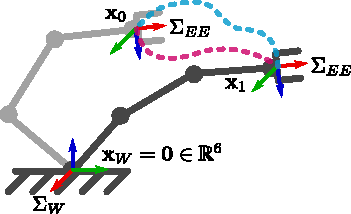
\includegraphics{images/manipulator_path.pdf}
            \caption{Cartesian paths illustration.}
    \end{figure}
    \end{minipage}%
    \begin{minipage}{.6\linewidth}
    \begin{itemize}
        \item $\mathbf{x}_0$ and $\mathbf{x}_1$ are EE poses w.r.t. $\mathbf{\Sigma}_W$
        \item Thanks to inverse kinematics, we can calculate $\mathbf{q}_1 = g(\mathbf{x}_1)$ 
        \item If we set this value to the motors, the robot will move towards that pose
        \item But...
        \begin{itemize}
            \item Which path will be followed?
            \item Which trajectory? 
            \item How can we control it? $\rightarrow$ Trajectory Planning
        \end{itemize}
    \end{itemize}
    \end{minipage}
    \end{center}

    \framebreak
    \begin{itemize}
        \item If there is an obstacle in the way of the robot, or if we want the robot to keep a specific orientation over the path (e.g., it carries a glass of water) $\Rightarrow$ \textcolor{uma_pink}{WE NEED A TRAJECTORY}
        \item \textbf{Generating the path:} Calculate a set of intermediate pose references (waypoints).
        \item \textbf{Generating the trajectory:} 
        \begin{enumerate}
            \item Set the arrival times to each of these waypoints.
            \item Define the polynomial to ensure a smooth trajectory.
        \end{enumerate}

        \vspace{0.5cm}
        \begin{figure}
            \centering
            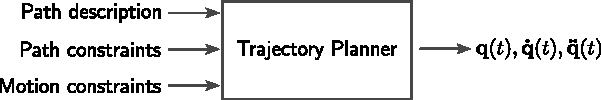
\includegraphics{images/trajectory_planner_schema.pdf}
            \caption{Trajectory planner diagram.}
            % \caption{Cartesian paths illustration.}
        \end{figure}
        
    \end{itemize}

    \framebreak
    Two trajectory Planning approaches:
    
    \begin{center}
    \begin{minipage}[t]{.5\linewidth}
        \textbf{\textcolor{uma_blue_dark}{Trajectories in the Joint Space:}}
        \begin{itemize}
            \item Planning in terms of controlled variables $(\mathbf{q}(t))$.
            \item A polynomial is generated for each joint.
            \item Lightweight computation.
            \item Easy to compute in real-time.
            \item Hard to determine the actual Cartesian motion.
            \item The EE trajectory is not controllable.
        \end{itemize}
    \end{minipage}
    \begin{minipage}[t]{.49\linewidth}
        \textbf{\textcolor{uma_blue_dark}{Trajectories in the Operational Space:}}
        \begin{itemize}
            \item Essential for tasks in the operational space.
            \item The EE Cartesian trajectory is known.
            \item Need to compute inverse kinematics (including $\mathbf{J}^{-1}$).
            \item Higher computational cost.
            \item Have to deal with singularities.
            \item The orientation is not unique.
            
        \end{itemize}
    \end{minipage}
    \end{center}

  
\end{frame}

\section{Trajectory Planning in the Joint Space}
\begin{frame}
	\frametitle{Outline} % Table of contents slide, comment this block out to remove it
	\tableofcontents[currentsection] % Throughout your presentation, if you choose to use \section{} and \subsection{} commands, these will automatically be printed on this slide as an overview of your presentation
\end{frame}


\begin{frame}[allowframebreaks]
\frametitle{Trajectory Planning in the Joint Space}

\textbf{\textcolor{uma_blue_dark}{Algorithm}}

\begin{minipage}[T!]{.48\linewidth}
\begin{algorithm}[H]
	$\mathbf{X} \gets \textsf{Knots}$\;
    $\mathbf{Q} = \textsf{inverse\_kinematics}(\mathbf{X})$\;
    $\mathcal{H}(t) \gets \mathcal{J}(\mathbf{Q}, t_f)$\;
    $t_k = 0$\;
	\While{$t_k < t_f$}
 	{
        $t_k = t_k + \Delta t$\;
        $\mathbf{q}_{d} = \mathcal{H}(t_k)$\;
        publish($\mathbf{q}_{d}$)\;
        sleep($\Delta t$);
  	}
\end{algorithm}
\end{minipage}
\begin{minipage}[T!]{.42\linewidth}
\begin{itemize}
    \item $\mathbf{X} = [\mathbf{x}_0, \dots, \mathbf{x}_l]\in\mathbb{R}^{6 \times l}$
    \item $\mathbf{Q} = [\mathbf{q}_0, \dots, \mathbf{q}_l]\in\mathbb{R}^{n \times l}$
    \item $\mathcal{J}\equiv$ polynomial interpolation.
    \item $l \equiv$ number of locations (knots).
    \item $t_k \equiv$ time at step $k$.
    \item $t_f \equiv$ final time.
    \item We get a trajectory for each joint (by interpolation).
    \item Not a Cartesian trajectory.
\end{itemize}
\end{minipage}

Different types of $\boldsymbol{h}(\mathbf{Q}, t_f)$ (already studied in Robot Programming and Control)~\cite{joint_trajectory_planning}:
\begin{itemize}
    \item Cubic polynomials, Quintic polynomials, Linear Segments with Parabolic Blends (LSPB)~\cite{point_to_point}.
\end{itemize}


\end{frame}

\section{Trajectory Planning in the Cartesian Space}
\begin{frame}
	\frametitle{Outline} % Table of contents slide, comment this block out to remove it
	\tableofcontents[currentsection] % Throughout your presentation, if you choose to use \section{} and \subsection{} commands, these will automatically be printed on this slide as an overview of your presentation
\end{frame}

\begin{frame}[allowframebreaks]
\frametitle{Trajectory Planning in the Operational Space}

\begin{itemize}
    \item We must schedule the Cartesian locations (poses) of the EE between the initial and final poses~\cite{cartesian_trajectory_planning}.
    \item The polynomial interpolation is conducted in the Operational Space (Cartesian interpolation):
    
    $
    \mathbf{h}(t_k) = \textsf{cartesian\_interpolation}(\mathbf{x}, t_f)\in\mathbb{R}^6
    $
    
    \item Position and Orientation along the generated Cartesian path must be defined separately (different representations).
    \item High actuators control frequency $\rightarrow$ real-time.
    \item The number of Cartesian locations (knots) to be interpolated in the Cartesian space is typically low (2 knots for point-to-point, 2 knots if using a via point).
    \item Simple interpolating paths in the Cartesian space (e.g., straight lines, arc of circles). Not necessary simple in the joint space.
\end{itemize}

\framebreak

\textbf{\textcolor{uma_blue_dark}{Algorithm}}

\begin{minipage}[T!]{.47\linewidth}
\begin{algorithm}[H]
	$\mathbf{X} \gets \textsf{Knots}$\;
    $\mathcal{H}(t) \gets \mathcal{C}(\mathbf{X}, t_f)$\;
    $t_k = 0$\;
	\While{$t_k < t_f$}
 	{
        $t_k = t_k + \Delta t$\;
        $\mathbf{x}_d = \mathcal{H}(t_k)$\;
        $\mathbf{q}_{d} =  \textsf{inverse\_kinematics}(\mathbf{x}_d)$\;
        publish($\mathbf{q}_{d}$)\;
        sleep($\Delta t$);
  	}
\end{algorithm}
\end{minipage}
\begin{minipage}[T!]{.42\linewidth}
\begin{itemize}
    \item $\mathcal{C}\equiv$ Cartesian interpolation.
    \item $l \equiv$ number of locations (knots).
    \item We get the Cartesian trajectory (by interpolation).
    \item We command the desired $\mathbf{q}_{d}$ obtained from kinematics inversion.
\end{itemize}
\end{minipage}
\end{frame}

% \begin{frame}[allowframebreaks]
% \frametitle{Methods for Cartesian Trajectory Planning}
% \begin{enumerate}
%     \item Bounded deviation joint paths.

%     \item Cartesian interpolation.
    
%     \begin{enumerate}
%         \item Homogeneous matrix interpolation.
%         \item Position interpolation
%         \item Orientation interpolation
%         \item Quaternions interpolation.
%         \item Smooth Cartesian trajectory planning.
%     \end{enumerate}
    

%     \item Optimal trajectory planning.
%     \begin{enumerate}
%         \item Dynamic scaling of the trajectories.
%     \end{enumerate}

%     % \item Optimal trajectory planning~\cite{vukobratovic1982method}.
% \end{enumerate}
% \end{frame}

\section{Bounded Deviation Joint Paths}
\begin{frame}
	\frametitle{Outline} % Table of contents slide, comment this block out to remove it
	\tableofcontents[currentsection] % Throughout your presentation, if you choose to use \section{} and \subsection{} commands, these will automatically be printed on this slide as an overview of your presentation
\end{frame}
\begin{frame}[allowframebreaks]
\frametitle{Bounded Deviation Joint Paths}

A hybrid Cartesian-joint approach: To follow a specific trajectory in the Cartesian space, one could define a series of via points (knots) and plan in the joint space.

A bounded deviation joint path defines enough knots to guarantee that the error (in Cartesian space) is bounded between admissible limits~\cite{taylor1979planning}.

 \begin{center}
    \begin{minipage}{.5\linewidth}
    \begin{figure}
        \centering
        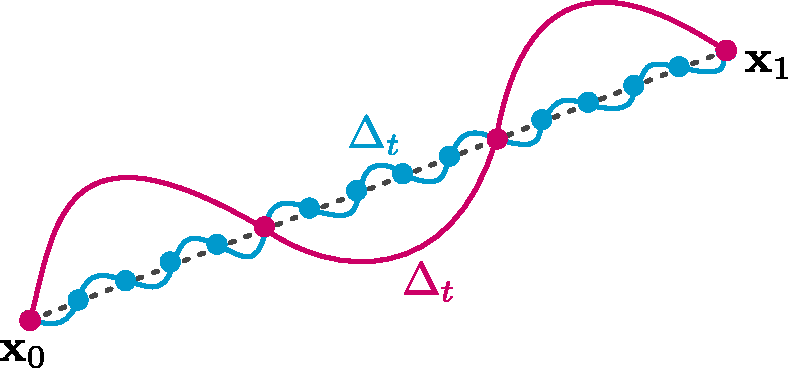
\includegraphics[width = 0.8\textwidth]{images/bounded_joint_path.pdf}
        \caption{Bounded deviation paths.}
    \end{figure}
    
    \begin{footnotesize}
        $\cdots$ Desired Cartesian path.
    
        \textcolor{uma_pink}{$-$ Bounded deviation path with few knots.}
    
        \textcolor{uma_blue_light}{$-$ Bounded deviation path with many knots.}    
    \end{footnotesize}
    
    \end{minipage}%
    \hspace{0.5cm}
    \begin{minipage}{.45\linewidth}
    \textcolor{uma_pink}{\textbf{Low number of knots:}}
        \begin{itemize}
            \item Low computation.
            \item High $\Delta_t$.
            \item High error.
        \end{itemize}
    \textcolor{uma_blue_light}{\textbf{High number of knots:}}
    \begin{itemize}
        \item High computation.
        \item Low $\Delta_t$.
        \item Low error.
    \end{itemize}
    \end{minipage}
\end{center}

    \framebreak

    \textbf{\textcolor{uma_blue_dark}{Recursive pre-planning method}}

    First, define the maximum position and orientation errors:
    $
    \delta_p^{\textsf{max}} = |p_j(t)-p_{j-1}(t-1)|, \, \delta_r^{\textsf{max}} = |\varphi|
    $
    \begin{enumerate}
        \item Calculate $\mathbf{q}_1$ and $\mathbf{q}_2$ (Inverse Kinematics).
        \item Compute the intermediate joint configuration $\mathbf{q}_i = \mathbf{q}_2-\frac{1}{2}\Delta\mathbf{q}_1$.
        \item Compute the intermediate Cartesian configuration $\mathbf{x}_i = \textsf{Forward Kinematics}(\mathbf{q}_i)$.
        \item Compute the bounded errors $\delta_p$ and $\delta_r$.
        \item Check the bounded errors $\delta_p \leq \delta_p^{\textsf{max}} $ and $\delta_r \leq \delta_r^{\textsf{max}}$.
        \item If the conditions are not satisfied, repeat steps 2 to 5 for the new segments created.
    \end{enumerate}

    Higher errors usually appear at the beginning and end of the trajectories (due to high velocity changes).
    


\end{frame}

\section{Cartesian Interpolation}
\subsection{Homogeneous Matrix Interpolation}
\begin{frame}
	\frametitle{Outline} % Table of contents slide, comment this block out to remove it
	\tableofcontents[currentsection,
        currentsubsection] % Throughout your presentation, if you choose to use \section{} and \subsection{} commands, these will automatically be printed on this slide as an overview of your presentation
\end{frame}

\begin{frame}[allowframebreaks]
\frametitle{Homogeneous Matrix Interpolation}

This method was proposed by Richard Paul~\cite{paul1979manipulator} to make up paths consist of straight line segments connected by smooth transitions with controlled acceleration.

\textcolor{uma_blue_dark}{\textbf{Concept}}
\begin{itemize}
    \item One of the simplest ways to change from one transform to the other is by a straight line translation and a rotation about same fixed axis in space.
    \item With such a line and axis then we can produce a motion of controlled linear and angular velocity.
    \item  However, the motion is made in terms of a translation and two rotations. The first rotation will serve to align the tool in the required final direction and the second rotation will control the orientation of the tool about the tool axis.
    \item As all manipulators end in a rotary joint, this second rotation in space corresponds to a rotation of the final joint of the manipulator. 
\end{itemize}

\framebreak


\begin{center}
    \begin{minipage}{.45\linewidth}
        \begin{figure}
            \centering
            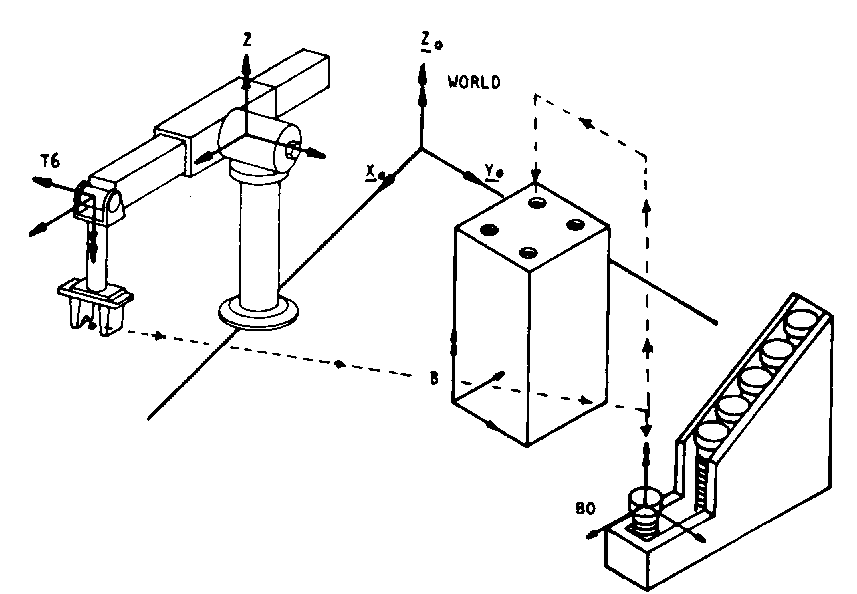
\includegraphics[width = 1\textwidth]{images/industrial_manipulator_task.pdf}
            \caption{Typical industrial manipulation task (source:~\cite{luh1983conventional}).}
        \end{figure}
    \end{minipage}%
    \hspace{0.5cm}
    \begin{minipage}{.5\linewidth}
    3 basic motions
    \begin{itemize}
        \item Translation: Linear displacement from $\mathbf{x}_A$ to $\mathbf{x}_B$.
        \item Rotation around translation axis: Ensuring Z-axis fo the EE and Z-axis of $\mathbf{x}_B$ are coincident.
        \item Rotation around Z-axis: Orient the EE (tool).  
    \end{itemize}
    \end{minipage}
\end{center}

\framebreak

\begin{figure}
    \centering
    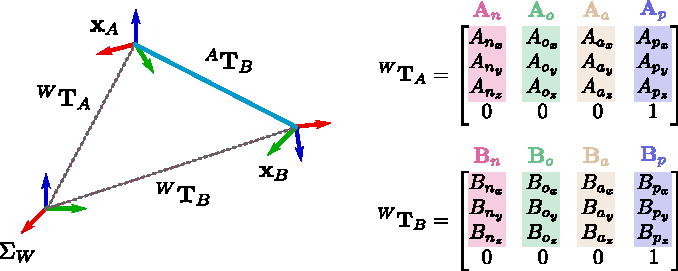
\includegraphics[width = 0.8\textwidth]{images/linear_segment.pdf}
    \caption{Linear segment representation between positions following the nomenclature in~\cite{paul1979manipulator}.}
\end{figure}

\framebreak

The homogeneous transformation between points $A$ and $B$ w.r.t. the world frame $W$ is defined as
$$
^A\mathbf{T}_B = \left[\begin{matrix}
    \mathbf{A}_n\mathbf{B}_n & \mathbf{A}_n\mathbf{B}_o & \mathbf{A}n\mathbf{B}_a & \mathbf{A}_{n}(\mathbf{B}_p - \mathbf{A}_p) \\
    \mathbf{A}_o\mathbf{B}_n & \mathbf{A}_o\mathbf{B}_o & \mathbf{A}o\mathbf{B}_a & \mathbf{A}_{o}(\mathbf{B}_p - \mathbf{A}_p) \\
    \mathbf{A}_a\mathbf{B}_n & \mathbf{A}_a\mathbf{B}_o & \mathbf{A}a\mathbf{B}_a & \mathbf{A}_{a}(\mathbf{B}_p - \mathbf{A}_p) \\
    0 & 0 & 0 & 1 \\
\end{matrix}\right]
$$
This transformation is the result of applying the three motions described above (one translation $\mathbf{T}$ and two rotations $\mathbf{R}_a$ and $\mathbf{R}_b$)
$$
^A\mathbf{T}_B = \mathbf{T} \mathbf{R}_a \mathbf{R}_b
$$

To achieve a desired Cartesian path, We can choose intermediate values of $^A\mathbf{T}_B $ representing a translation and two rotations. To achieve a linear segment (linear interpolation) we will choose intermediate values $h$ of $^A\mathbf{T}_B$, where $h\in\mathbb{R} : 0\leq h \leq 1$. 

\framebreak

The translation will be along the line joining $A$ and $B$ and will be represented by the transformation $T(h)$. The first rotation will serve to rotate the approach vector, the direction in which the tool is pointing, from $A$ into the approach vector at $B$. This rotation will be represented by $R_a(h)$. The second rotation will rotate the orientation vector, representing the orientation of the tool, from $A$ into the orientation vector at $B$, $R_o(h)$. We will then represent $^A\mathbf{T}_B(h)$ as

$$
^A\mathbf{T}_B(h) = \mathbf{T}(h) \mathbf{R}_a(h) \mathbf{R}_b(h)
$$

Then, if $h=0 \implies ^A\mathbf{T}_B(0) = ^W\mathbf{T}_A$ and $h=1 \implies ^A\mathbf{T}_B(1) = ^W\mathbf{T}_B$.



\framebreak 

This way, varying $h$ linearly over time, the EE of the manipulator will follow a perfect linear trajectory in the Cartesian space.

According to this, both the translation and rotations will be directly proportional to $h$ so that if $h$ varies linearly with respect to time,  the motion represented by $^A\mathbf{T}_B(h)$ will correspond to a constant linear and two constant angular velocities. 
\end{frame}

\subsection{Interpolation of the Position}
\begin{frame}
	\frametitle{Outline} % Table of contents slide, comment this block out to remove it
	\tableofcontents[currentsection,
        currentsubsection] % Throughout your presentation, if you choose to use \section{} and \subsection{} commands, these will automatically be printed on this slide as an overview of your presentation
\end{frame}
\begin{frame}[allowframebreaks]
\frametitle{Interpolation of the Position}

The interpolation of the position is straightforward by defining a straight line joining $A$ and $B$ (path) interpolated over time (trajectory)

$$
^A\mathbf{T}_B(h) = \left[\begin{matrix}
     &   &  & hx \\
     &  \mathbf{I}_{3 \times 3} &  & hy \\
     &   &  & hz \\
     & \mathbf{0}_{1 \times 3} &  & 1 \\
\end{matrix}\right] =
\left[\begin{matrix}
     &   &  & hx \\
     &  \mathbf{I}_{3 \times 3} &  & hy \\
     &   &  & hz \\
     & \mathbf{0}_{1 \times 3} &  & 1 \\
\end{matrix}\right]
$$

\end{frame}

\subsection{Interpolation of the Orientation}
\begin{frame}
	\frametitle{Outline} % Table of contents slide, comment this block out to remove it
	\tableofcontents[currentsection,
        currentsubsection] % Throughout your presentation, if you choose to use \section{} and \subsection{} commands, these will automatically be printed on this slide as an overview of your presentation
\end{frame}
\begin{frame}[allowframebreaks]
\frametitle{Interpolation of the Orientation}


\end{frame}


\subsection{Smooth Cartesian Trajectory Planning}
\begin{frame}
	\frametitle{Outline} % Table of contents slide, comment this block out to remove it
	\tableofcontents[currentsection,
        currentsubsection] % Throughout your presentation, if you choose to use \section{} and \subsection{} commands, these will automatically be printed on this slide as an overview of your presentation
\end{frame}
\begin{frame}[allowframebreaks]
\frametitle{Smooth Cartesian Trajectory Planning}


Nowadays, we keep studying this~\cite{tagliavini2023smooth}.

\end{frame}


\section{Optimal Trajectory Planning}
\begin{frame}
	\frametitle{Outline} % Table of contents slide, comment this block out to remove it
	\tableofcontents[currentsection,
        currentsubsection] % Throughout your presentation, if you choose to use \section{} and \subsection{} commands, these will automatically be printed on this slide as an overview of your presentation
\end{frame}
\begin{frame}[allowframebreaks]
\frametitle{Optimal Trajectory Planning}

~\cite{vukobratovic1982method}

\end{frame}


\begin{frame}[allowframebreaks]
\frametitle{Dynamic Scaling of Trajectories}

~\cite{hollerbach1983dynamic}

\end{frame}




\begin{frame}[allowframebreaks]
\frametitle{Bibliography}
\printbibliography
\end{frame}

\end{document}